The developed mathematical model comprised of Eqs. \ref{eq:pde_mg}, \ref{eq:pde_film}, \ref{eq:pde_cl}, \ref{eq:pde_oh}, and \ref{eq:lsm_final} cannot be solved using analytical techniques. The alternative approach in these scenarios is solving the derived PDEs numerically. In \biodeg{}, we used a combination of finite element and finite difference methods to solve the aforementioned equations. In the developed numerical model, the PDEs are solved one by one, each of which is a linear equation, so the model implementation follows the principles of solving linear systems. In the following section, only the process to obtain the solution of Eq. \ref{eq:pde_mg} is described in detail, but the other PDEs were solved using the same principle. 

\subsection{Finite element formulation}

In order to solve Eq. \ref{eq:pde_mg} numerically, we used a finite difference scheme for the temporal term and a finite element formulation for the spatial terms. For simplicity of writing, notations of variables are changed, so $C_\mathrm{Mg}$ is represented as $u$ (the main unknown state variable to find), $C_\mathrm{Film}$ is denoted by $p$, $C_\mathrm{Cl}$ is denoted by $q$, and the saturation term $(1-\frac{F}{F_{\max }})$ is denoted by $s$. By doing this, Eq. \ref{eq:pde_mg} can be written as
\begin{equation} \label{eq:pde_changed_not}
\frac{\partial u}{\partial t}=\nabla \cdot (D   \nabla u)-k_{1} s u+k_{2} p q^{2}.
\end{equation}

To obtain the finite element formulation, the weak form of derived PDE is required. In order to get this, we define a space of test functions and then, multiply each term of the PDE by any arbitrary function as a member of this space. The test function space is
\begin{equation} \label{eq:function_space}
\mathcal{V}=\left\{v(\mathbf{x}) | \mathbf{x} \in {\Omega}, v(\mathbf{x}) \in \mathcal{H}^{1}(\Omega), \text { and } v(\mathbf{x})=0 \text { on } \Gamma\right\}
\end{equation}
in which the $\Omega$ is the domain of interest, $\Gamma$ is the boundary of $\Omega$, and $\mathcal{H}^{1}$ denotes the Sobolev space of the domain $\Omega$, which is a space of functions whose derivatives are square-integrable functions in $\Omega$. The solution of the PDE belongs to a trial function space, which is similarly defined as
\begin{equation} \label{eq:trial_domain}
\mathcal{S}_{t}=\left\{u(\mathbf{x}, t) | \mathbf{x} \in \Omega, t>0, u(\mathbf{x}, t) \in \mathcal{H}^{1}(\Omega), \text { and } \frac{\partial u}{\partial n}=0 \text { on } \Gamma\right\}.
\end{equation}

Then, we multiply Eq. \ref{eq:pde_changed_not} to an arbitrary function $v \in \mathcal{V}$:

\begin{equation}
\frac{\partial u}{\partial t} v=\nabla \cdot (D  \nabla u) v-k_{1} s u v+k_{2} p q^{2} v.
\end{equation}

\noindent Integrating over the whole domain yields:
\begin{equation} \label{eq:int_first}
\int_{\Omega} \frac{\partial u}{\partial t} v d \omega=\int_{\Omega} \nabla \cdot (D  \nabla u) v d \omega-\int_{\Omega} k_{1} s u v d \omega+\int_{\Omega} k_{2} p q^{2} v d \omega.
\end{equation}

\noindent The diffusion term can be split using the integration by parts technique:
\begin{equation} \label{eq:int_part}
\int_{\Omega} \nabla \cdot (D  \nabla u) v d \omega = \int_{\Omega} \nabla \cdot[v(D  \nabla u)] d \omega-\int_{\Omega} (\nabla v) \cdot(D  \nabla u) d \omega
\end{equation}

\noindent in which the second term can be converted to a surface integral on the domain boundary by applying the Green's divergence theory:
\begin{equation} \label{eq:divergence}
\int_{\Omega} \nabla \cdot[v(D  \nabla u)] d \omega = \int_{\Gamma} D v \frac{\partial u}{\partial n} d \gamma.
\end{equation}

\noindent For the temporal term, we use the finite difference method and apply a first-order backward Euler scheme for discretization, which makes it possible to solve the PDE implicitly:
\begin{equation} \label{eq:backward}
\frac{\partial u}{\partial t} = \frac{u-u^{n}}{\Delta t}
\end{equation}
\noindent where $u^n$ denotes the value of the state variable in the previous time step (or initial condition for the first time step). Inserting Eqs. \ref{eq:int_part}, \ref{eq:divergence}, and \ref{eq:backward} into Eq. \ref{eq:int_first} yields:
\begin{equation}
\int_{\Omega} \frac{u-u^{n}}{\Delta t} v d \omega=\int_{\Gamma} D v  \frac{\partial u}{\partial n} d \gamma-\int_{\Omega} D  \nabla u \cdot \nabla v d \omega-\int_{\Omega} k_{1} s u v d \omega+\int_{\Omega} k_{2} p q^{2} v d \omega.
\end{equation}

\noindent The surface integral is zero because there is a no-flux boundary condition on the boundary of the computational domain (defined in the trial function space according to Eq. \ref{eq:trial_domain}). By reordering the equation, we get the weak form of Eq. \ref{eq:pde_changed_not}:
\begin{equation}  \label{eq:weak_general}
\int_{\Omega} {u} v d \omega+\int_{\Omega} \Delta t D  \nabla u \cdot  \nabla v d \omega+\int_{\Omega} \Delta tk_{1} s u v d \omega=\int_{\Omega} {u^{n}} v d \omega+\int_{\Omega} \Delta t k_{2} p q^{2} v d \omega.
\end{equation}

%\begin{equation}  \label{eq:weak_general}
%\int_{\Omega} \frac{u}{\Delta t} v d \omega+\int_{\Omega} D \cdot \nabla \cdot u \nabla v d \omega+\int_{\Omega} k_{1} s u v d \omega=\int_{\Omega} \frac{u^{n}}{\Delta t} v d \omega+\int_{\Omega} k_{2} p q^{2} v d \omega
%\end{equation}

%\begin{equation}
%\begin{aligned} \int_{\Omega} \frac{[\mathrm{Mg}]}{\Delta t} v d \omega+\int_{\Omega} & D \cdot \nabla[\mathrm{Mg}] \cdot \nabla v d \omega+\int_{\Omega} k_{1}[\mathrm{Mg}] v d \omega-\int_{\Omega} k_{1}[\mathrm{Mg}]\left(\frac{F}{F_{\mathrm{max}}}\right) v d \omega \\ &=\int_{\Omega} \frac{[\mathrm{Mg}]^{\mathrm{old}}}{\Delta t} v d \omega+\int_{\Omega} k_{2}[F][\mathrm{Cl}]^{2} v d \omega \end{aligned}
%\end{equation}


So, the problem is to find a function $u(t) \in \mathcal{S}_{t}$ such that for all $v \in \mathcal{V}$ Eq. \ref{eq:weak_general} would be satisfied. By defining a linear functional $(f, v) =\int_{\Omega} f v d \omega$ and encapsulating the independent concentration terms into $f^{n} = pq^2$, Eq. \ref{eq:weak_general} can be simplified as:
\begin{equation}
(u, v)[1+\Delta t k_1 s]+\Delta t(D \nabla u, \nabla v)=\left(u^{n}, v\right)+\Delta t\left(f^{n}, v\right)
\end{equation}
and so as 
\begin{equation}
(u, v)+\Delta t(D \nabla u, \nabla v)+\Delta t k_1 b (u, v)=\left(u^{n}, v\right)+\Delta t\left(f^{n}, v\right)
\end{equation}



\noindent which can be further converted to the common form of the weak formulation of time-dependent reaction-diffusion PDEs by multiplying to a new coefficient $\alpha = \frac{1}{1+\Delta t k_1 s}$:

\begin{equation} \label{eq:weak_compact}
(u, v)+ \alpha \Delta t(D \nabla u, \nabla v)=\alpha \left(u^{n}, v\right)+ \alpha \Delta t\left(f^{n}, v\right).
\end{equation}

One can approximate the unknown function $u$ in Eq. \ref{eq:weak_compact} by $u(x) \approx \sum_{i=0}^{N} c_{i} \psi_{i}(x)$, where the $\psi_{i}$ are the basis functions used to discretize the function space, and $c_0,\ldots,c_N$ are the unknown coefficients. The finite element method uses Lagrange polynomials as the basis function and discretizes the computational domain using a new function space $\mathcal{V}_h$ spanned by the basis functions $\left\{\psi_{i}\right\}_{i \in \mathcal{I}_{s}}$, in which $\mathcal{I}_{s}$ is defined as $\mathcal{I}_{s}=\{0, \ldots, N\}$, where $N$ denotes the degrees of freedom in the computational mesh. The computational mesh discretizes the space into a finite number of elements, in each of which the $\psi_{i}$ is non-zero inside the $i$th element and zero everywhere else. In \biodeg{}, 1st order Lagrange polynomials were used as the basis functions to define the finite element space.

For 1D elements, a 1st order Lagrange polynomial for the $i$th element with the width of $h$ can be written as:
\begin{equation}
\psi_{i}(x)=\left\{\begin{array}{cc}{0} & {\quad x<x_{i-1}} \\ {\left(x-x_{i-1}\right) / h} & {\quad x_{i-1} \leq x<x_{i}} \\ {1-\left(x-x_{i}\right) / h} & {\quad x_{i} \leq x<x_{i+1}} \\ {0} & {\quad x \geq x_{i+1}}\end{array}\right. .
\end{equation}

A similar approach can be applied to define the basis function space in 2D and 3D spaces.

In order to derive a linear system of equations for obtaining the unknown coefficients $c_j$, we define
\begin{equation} \label{eq:u_definition}
u=\sum_{j=0}^{N} c_{j} \psi_{j}(\boldsymbol{x}), \quad u^{n}=\sum_{j=0}^{N} c_{j}^{n} \psi_{j}(\boldsymbol{x})
\end{equation}

\noindent as the definition of the unknown function $u$ and its value in the previous time step $u^n$. We then insert it into Eq. \ref{eq:weak_compact}, which yields the following equation for each degree of freedom $i=0, \ldots, N$, where the test functions are selected as $v = \psi_i$:
\begin{equation} \label{eq:weak_sum_all}
\sum_{j=0}^{N}\left(\psi_{i}, \psi_{j}\right) c_{j} + \alpha \Delta t \sum_{j=0}^{N}\left(\nabla \psi_{i}, D \nabla \psi_{j}\right) c_{j} =\sum_{j=0}^{N} \alpha \left(\psi_{i}, \psi_{j}\right) c_{j}^{n}+\alpha\Delta t\left(f^{n}, \psi_{i}\right).
\end{equation}

Eq. \ref{eq:weak_sum_all} is a linear system
\begin{equation} \label{eq:linear_system}
\sum_{j} A_{i, j} c_{j}=b_{i}
\end{equation}
with
\begin{equation} \label{eq:system_a}
A_{i, j}=\left(\psi_{i}, \psi_{j}\right) + \alpha \Delta t \left(\nabla \psi_{i}, D \nabla \psi_{j}\right)
\end{equation}
\begin{equation} \label{eq:system_b}
b_{i}=\sum_{j=0}^{N}\alpha \left(\psi_{i}, \psi_{j}\right) c_{j}^{n}+\alpha \Delta t\left(f^{n}, \psi_{i}\right)
\end{equation}

\noindent which can be rewritten as
\begin{equation} \label{eq:linear_eq_simple}
(M+\alpha \Delta t K) c=\alpha M c_{1}+\alpha \Delta t f.
\end{equation}

$M$ (which traditionally is called the mass matrix), $K$ (which traditionally is called the stiffness matrix), $f$, $c$, and $c_1$ are defined as
\begin{equation} \label{eq:matrices_defintion}
\begin{aligned} M &=\left\{M_{i, j}\right\}, \quad M_{i, j}=\left(\psi_{i}, \psi_{j}\right), \quad i, j \in \mathcal{I}_{s} \\ K &=\left\{K_{i, j}\right\}, \quad K_{i, j}=\left(\nabla \psi_{i}, D \nabla \psi_{j}\right), \quad i, j \in \mathcal{I}_{s} \\ f &=\left\{f_{i}\right\}, \quad f_{i}=\left(f\left(\boldsymbol{x}, t_{n}\right), \psi_{i}\right), \quad i \in \mathcal{I}_{s} \\ c &=\left\{c_{i}\right\}, \quad i \in \mathcal{I}_{s} \\ c_{1} &=\left\{c_{i}^{n}\right\}, \quad i \in \mathcal{I}_{s} \end{aligned}
\end{equation}

By solving Eq. \ref{eq:linear_system} and substituting the obtained $c$ in Eq. \ref{eq:u_definition}, $u$ ($C_{\mathrm{Mg}}$ in this example) can be calculated in the current time step. As stated before, the same approach can be applied to Eq. \ref{eq:pde_film} and Eq. \ref{eq:lsm_final} to get $C_{\mathrm{Film}}$ and $\phi$. This procedure is repeated in each time step to compute the values of $C_{\mathrm{Mg}}$, $C_{\mathrm{Film}}$, and $\phi$ over time.

A common practice to save time for solving Eq. \ref{eq:linear_system}  for a constant time step size is to compute the left-hand side matrix ($A$ in Eq. \ref{eq:system_a}) once and compute only the right-hand side vector of the equation at each time iteration. But in this case, although the time step size is fixed, due to the presence of the $\alpha$ coefficient, the matrix changes along the time. The $\alpha$ coefficient is not constant and should be updated in each time step because it depends on the penalization term $s$ (which is a function of the concentration of the film as can be seen by comparing Eq. \ref{eq:pde_mg} and Eq. \ref{eq:pde_changed_not}). In addition to this, the diffusion coefficient is not constant (Eq. \ref{eq:diff_coeff}), making the second term in Eq. \ref{eq:system_a} non-constant even in the absence of $\alpha$ coefficient. Consequently, the left-hand side matrix of the Eq. \ref{eq:linear_system} cannot be computed before the start of the main time loop, and computing it in each time step is an extra but inevitable computational task in comparison to similar efficient and high-performance finite element implementations. This contributes to a slower algorithm for solving the aforementioned PDEs.

\subsection{Implementation and parallelization}

The model was implemented in FreeFEM \cite{Hecht2012}, which is an open-source PDE solver to facilitate converting the weak formulation (Eq. \ref{eq:weak_general}) to a linear system $Ax=b$ (with $A$ from Eq. \ref{eq:system_a} and $b$ from Eq. \ref{eq:system_b}). 

Computing the diffusion solely in the medium domain causes oscillations close to the interface, and to prevent this, the mass lumping feature of FreeFEM was employed. In this technique, the desired mass matrix is handled node-wise and not element-wise. Technically speaking, this means that the state variable is stored in the mesh nodes, and although this is the natural formulation in the finite difference method, it requires artificial modification in the standard finite element formulation \cite{Wendland2005}. The mass lumping feature of FreeFEM applies a quadratic formula at the vertices of elements to make the mass matrix diagonal, which contributes positively to the convergence of the solution.


The main parallelization approach in \biodeg{} was domain decomposition, in which the mesh is split into smaller domains (can be overlapping or non-overlapping), and the global solution of the linear system is achieved by solving the problem on each smaller local mesh. What really matters in this approach is providing virtual boundary conditions to the smaller sub-domains by ghost elements, transferring neighboring sub-domain solutions \cite{Badri2018}. As a result, a high-performance parallelism is feasible by assigning each sub-domain to one processing unit.

In computational science, preconditioning is widely used to enhance the convergence, which means instead of directly working with a linear system $Ax=b$, one can consider the preconditioned system \cite{Daas2019AMS}:
\begin{equation} \label{eq:precond_system}
M^{-1} A x=M^{-1} b
\end{equation}
in which the $M^{-1}$ is the preconditioner. In \biodeg{}, we considered this approach for both the domain composition and the solution of the linear system. We opted to use an overlapping Schwarz method for domain decomposition, in which the mesh is first divided into a graph of $N$ non-overlapping meshes using METIS (or ParMETIS) \cite{METIS1998}. Then, by defining a positive number $\delta$, the overlapping decomposition $\left\{\mathcal{T}_{i}^{\delta}\right\}_{1 \leqslant i \leqslant N}$ can be created recursively for each sub-mesh $\left\{\mathcal{T}_{i}\right\}_{1 \leqslant i \leqslant N}$ by adding all adjacent elements of $\mathcal{T}_{i}^{\delta-1}$ to it. Then, the finite element space $\mathcal{V}_{h}$ (Eq. \ref{eq:function_space}) can be mapped to the local space $\left\{\mathcal{V}_{i}^{\delta}\right\}_{1 \leqslant i \leqslant N}$ by considering the restrictions $\left\{R_{i}\right\}_{1 \leqslant i \leqslant N}$ and a local partition of unity $\left\{D_{i}\right\}_{1 \leqslant i \leqslant N}$ such that:
\begin{equation} \label{eq:restrict}
\sum_{j=1}^{N} R_{j}^{\top} D_{j} R_{j}=I_{n \times n}
\end{equation}
where $I$ and $n$ denote identity matrix and the global number of unknowns, respectively \cite{Dolean2015}.

In \biodeg{}, we decomposed the mesh by using the one-level preconditioner Restricted Additive Schwarz (RAS):
\begin{equation} \label{eq:ras}
M_{\mathrm{RAS}}^{-1}=\sum_{i=1}^{N} R_{i}^{\top} D_{i} A_{i}^{-1} R_{i}
\end{equation}
in which $\left\{A_{i}\right\}_{1 \leqslant i \leqslant N}$ is the local operator of the sub-matrices \cite{Dolean2015}. For this purpose, we took advantage of the HPDDM (high-performance domain decomposition methods) package interface in FreeFEM \cite{Jolivet2013}. The partitioned mesh is shown in Fig. \ref{fig:overlap}. The effect of the construction of these local sub-domains on the sparsity pattern of the global matrix is also depicted in Fig. \ref{fig:sparsity_pattern}. The global matrix is a sparse matrix according to Eq. \ref{eq:system_a} and the definition of the basis function $\psi$.

\begin{figure}[ht]
\center 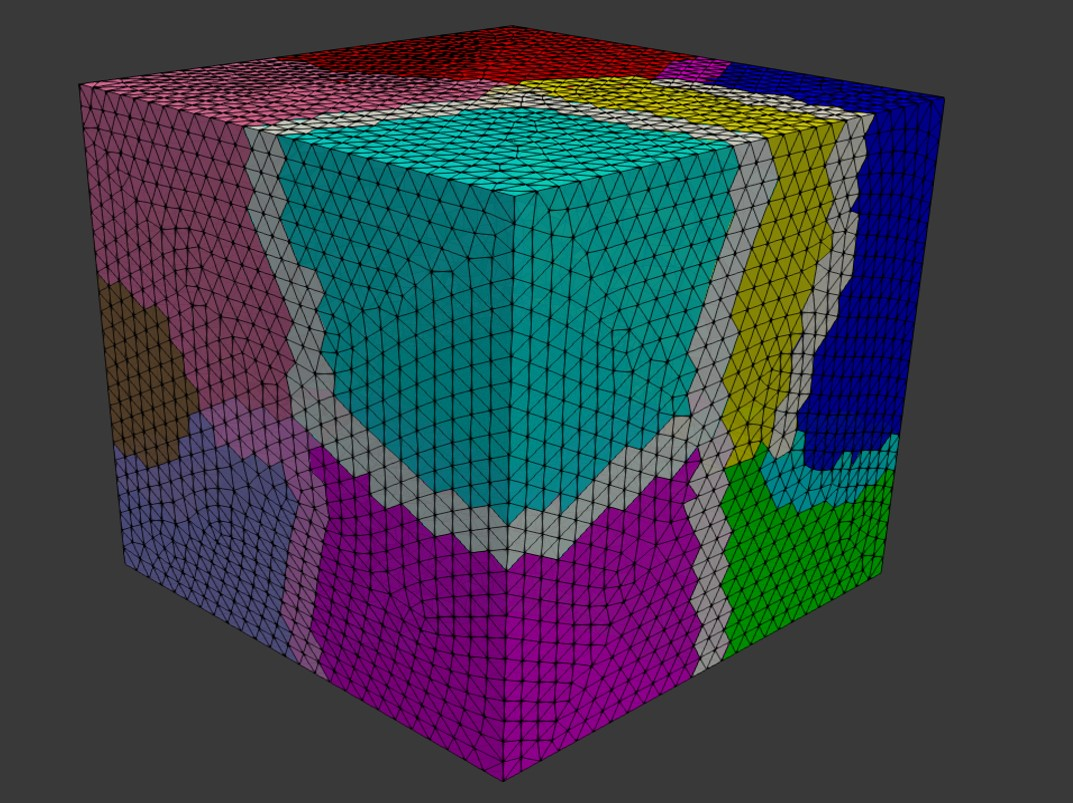
\includegraphics[width=6cm]{overlap}
\caption{Overlapping domain decomposition in \biodeg{}. Each color shows a separate sub-domain, and the narrow lighter bands are the overlapped regions.} \label{fig:overlap}
\end{figure}


\begin{figure}[ht]
\center 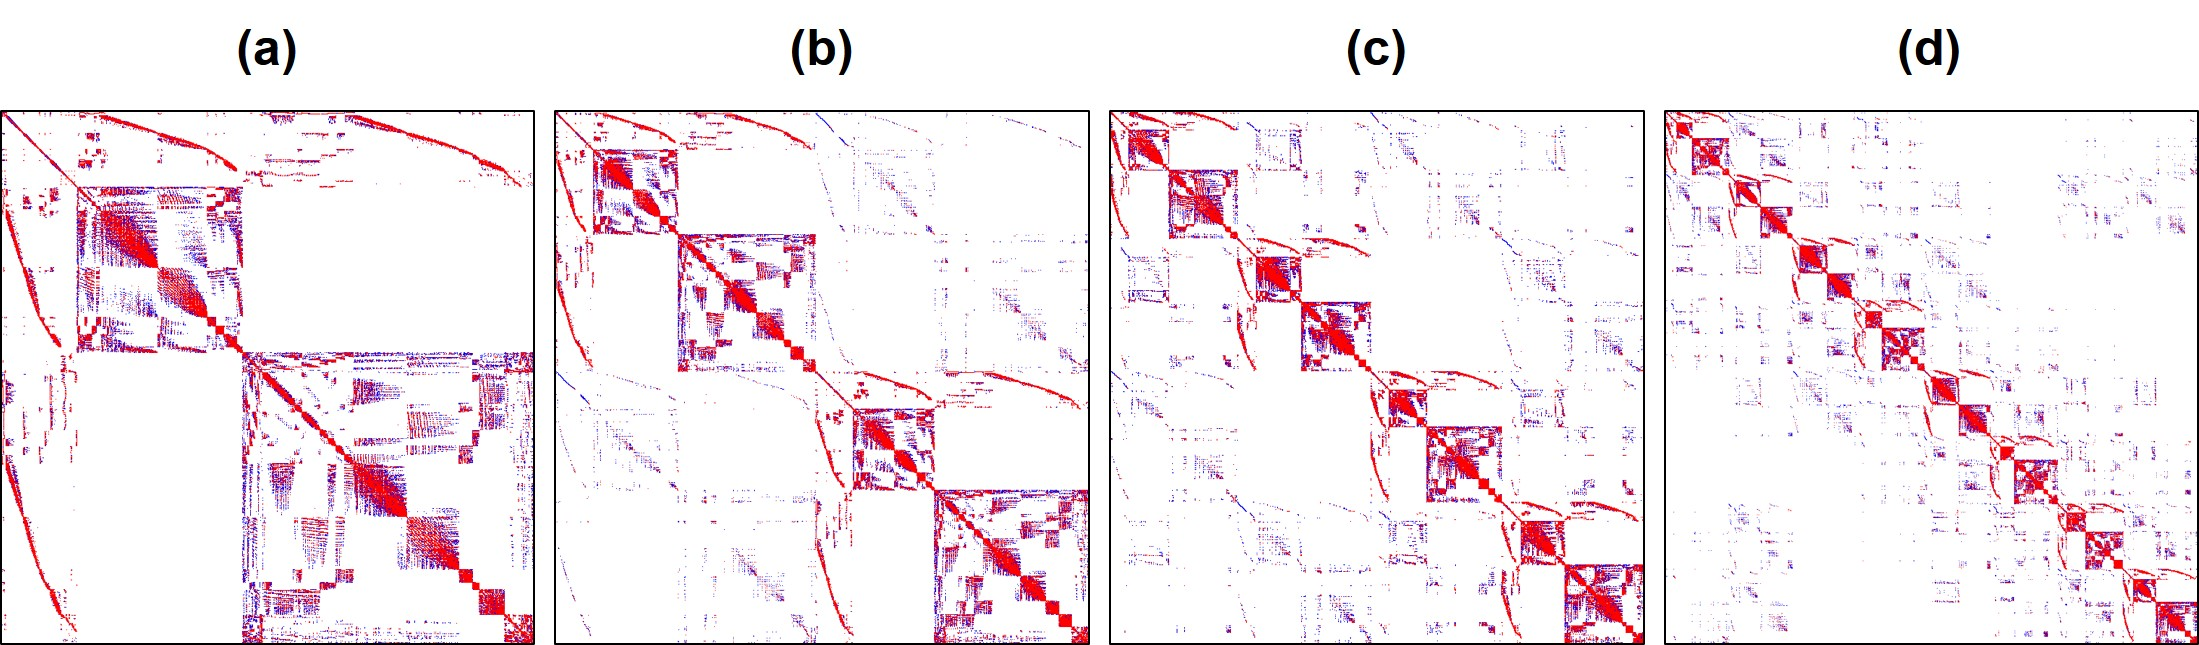
\includegraphics[width=12cm]{sparsity_pattern}
\caption{Comparison of the sparsity patterns (highlighting non-zero elements) of the global matrix A for a different number of decomposed domains a: 1 domain b: 2 sub-domains c: 4 sub-domains d: 8 sub-domains.} \label{fig:sparsity_pattern}
\end{figure}


Generally, two categories of methods have been used to solve a large linear system of equations on parallel machines: direct solvers (e.g. Multifrontal Massively Parallel Sparse, MUMPS \cite{MUMPS1}) and iterative solvers (e.g. Generalized Minimal Residual Method, GMRES \cite{Saad1986}). While direct solvers are quite robust, they suffer from the memory requirement problem on large systems. Inversely, iterative solvers are quite efficient on memory consumption, but similar to other iterative approaches, they are not very reliable in some cases \cite{Saad2003}. Direct solvers modify the matrix by factorization (e.g. Cholesky decomposition), but an iterative solver does not manipulate the matrix and works solely using basic algebraic operations. However, for an efficient usage of iterative solvers, a proper preconditioner is crucial \cite{Saad2003}. By evaluating and comparing the performance of the aforementioned methods for the current model, we decided to use an iterative approach using the Krylov subspaces (KSP) method, in which we preconditioned the equation using a proper preconditioner (Eq. \ref{eq:precond_system}) and then solved it with an iterative solver.

Krylov methods have been frequently used by researchers as robust iterative approaches to parallelism \cite{Ipsen1998}. What matters in this regard is ensuring proper scaling of the parallelized algorithm for both the assembling of the matrices and the solution of the linear system of equations. One good solution to this challenge is taking advantage of HPC-ready mathematical libraries to achieve efficient distributed-memory parallelism through the Message Passing Interface (MPI). In \biodeg{}, we used the PETSc (Portable, Extensible Toolkit for Scientific Computation) library \cite{petsc}, which provides a collection of high-performance preconditioners and solvers for this purpose.

In order to yield the highest performance, a variety of different combinations of KSP types and preconditioners were evaluated, and the best performance for the reaction-diffusion system model was achieved using the HYPRE BoomerAMG preconditioner \cite{Falgout2002} and the GMRES solver \cite{Saad1986}. 